% This text is proprietary.
% It's a part of presentation made by myself.
% It may not used commercial.
% The noncommercial use such as private and study is free
% Nov. 2006
% Author: Sascha Frank
% University Freiburg
% www.informatik.uni-freiburg.de/~frank/
%
% additional usepackage{beamerthemeshadow} is used
%
%  \beamersetuncovermixins{\opaqueness<1>{25}}{\opaqueness<2->{15}}
%  with this the elements which were coming soon were only hinted
\documentclass{beamer}
\usepackage{beamerthemeshadow}
\usepackage{amssymb}
\usepackage{multirow}
\DeclareMathOperator*{\argmin}{\arg\!\min}

\renewcommand{\vec}[1]{\boldsymbol{#1}}
\newcommand{\mat}[1]{\text{\bf #1}}

\usetheme{Berlin}

\setbeamertemplate{footline}[page number] % add page number
\setbeamertemplate{navigation symbols}{}  % remove bottom buttons.
\setbeamertemplate{headline}{} % remove section from header.

%\renewcommand{\labelitemii}{$\diamondsuit$}

\definecolor{orange}{RGB}{255,127,0}
\definecolor{ForestGreen}{RGB}{34,139,34}
\definecolor{Red}{RGB}{255,0,0}

\begin{document}
\title[4D Active Cut]{4D Active Cut: An Interactive Tool for Pathological Anatomy Modeling}
\author[Wang, Liu, Prastawa, Irimia, Vespa, Van Horn, Fletcher, Gerig]{Bo Wang $^{\text{a,b}}$, Wei Liu $^{\text{a,b}}$, Marcel Prastawa $^{\text{a,b}}$, Andrei Irimia $^{\text{c}}$, Paul M. Vespa $^{\text{d}}$, John D. Van Horn $^{\text{c}}$, P. Thomas Fletcher $^{\text{a,b}}$, and Guido Gerig $^{\text{a,b}}$}
\institute[SCI UTAH, INI USC and others]{
  $^{\text{a}}$ Scientific Computing and Imaging Institute, \\
  $^{\text{b}}$ School of Computing, University of Utah \\
  $^{\text{c}}$ Institute for Neuroimaging and Informatics, University of Southern California \\
  $^{\text{d}}$ Brain Injury Research Center, University of California, Los Angeles.
}
\date[Imaging Lunch Presentation]{Imaging Lunch - Dec. 9, 2013}

\frame{\titlepage}

\frame{\frametitle{Table of contents}\tableofcontents}


\section{Motivation and Background}
\subsection{Motivation of TBI imaging research}
\frame{\frametitle{Motivation}
\begin{itemize}
\item 4D pathological anatomy modeling is key to understanding complex
pathological brain images.
\item It is a challenging problem due to the difficulties
in detecting multiple appearing and disappearing lesions across time points and estimating
dynamic changes and deformations between them.
\item Existing
interactive segmentation methods passively waits for user to refine the
segmentations which is a difficult task in 3D images that change over time.
\end{itemize}
}

\frame{\frametitle{TBI images}
\begin{figure}
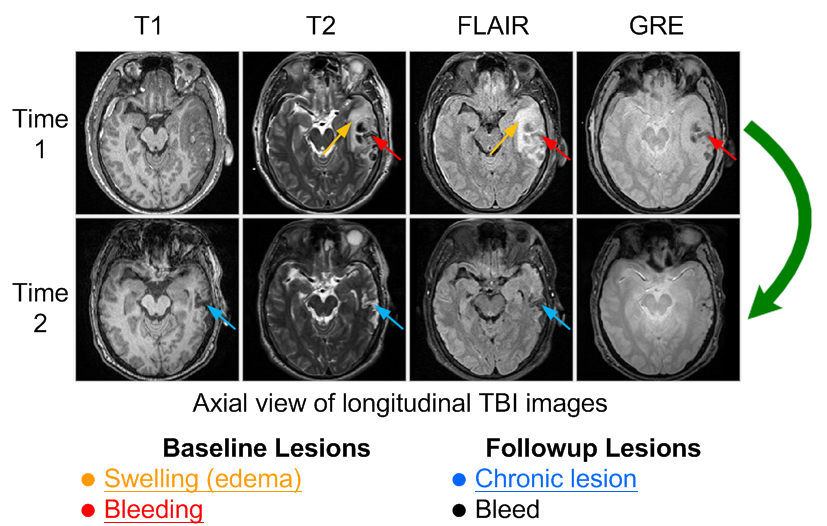
\includegraphics[scale=0.8]{./images/TBI_data_sml.png}
\end{figure}
}

\frame{\frametitle{4D modeling enables other analysis}
Structural pathology analysis
\begin{center}
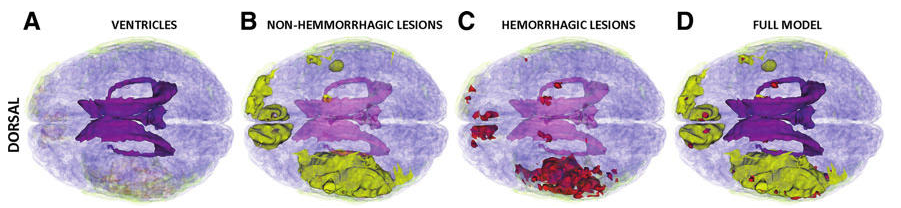
\includegraphics[width=1.0\textwidth]{./images/structural_analysis.PNG}\\
{\scriptsize \textcolor{ForestGreen}{Andrei Irimia et al., Journal of Neurotrauma, 2011}}
\end{center}
Brain connectivity analysis
\begin{center}
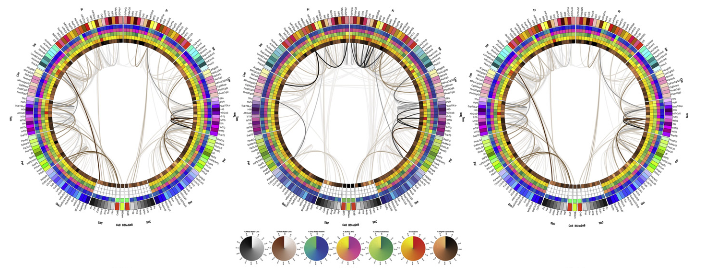
\includegraphics[width=0.8\textwidth]{./images/connectivity.PNG}\\
{\scriptsize \textcolor{ForestGreen}{Andrei Irimia et al., NeuroImage: Clinical, 2012}}
\end{center}
}


\subsection{Previous work}
\frame{\frametitle{GrabCut interactive segmentation method}
GrabCut, \textcolor{ForestGreen}{Carsten Rother et al., ACM TOG 2004}\\
\begin{itemize}
\item User gives an initial guess of the region of interest (foreground).
\item The algorithm estimates globally optimal boundary between the foreground and background regions.
\item The user then inspects
the segmentation results, and adjusts the boundary by drawing
a region as a hard constraint.
\end{itemize}
This process works well on 2D images, as users can quickly find incorrectly classified regions.\\
\textcolor{Red}{However, such interaction is a huge burden to users
once applied to 3D volume data, since one has to visually
inspect each slice and correct it.}
}

\frame{\frametitle{GrabCut algorithm}
\begin{itemize}
  \item User gives bounding box (trimap) to initialize the algorithm which is used for initial $\alpha$ map. \\
  Begin: iterative minimization
  \begin{enumerate}
    \item Assign Gaussian mixture models(GMM) components to pixels using current $\alpha$ map.
    \item Learn GMM parameters from data.
    \item Estimate Segmentation using the Graph Cut based on the estimated GMM parameters to update $\alpha$ map.
    \item Repeat 1-3, until convergence.
  \end{enumerate}
  End: iterative minimization
  \item User editing
\end{itemize}
}

\frame{\frametitle{GrabCut interactive segmentation method}
    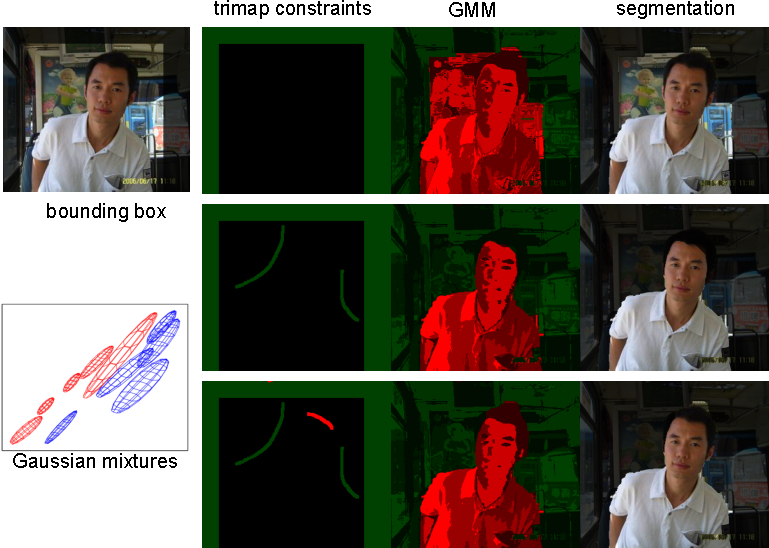
\includegraphics[width=0.9\textwidth]{images/grabcut/gc.pdf}
}

\frame{\frametitle{GrabCut interactive segmentation method}
The disadvantages of GrabCut or similar methods:
\begin{itemize}
\item The algorithm is in a passive
learning state.
\item Its performance entirely depends on user's
active inspection and correction.
\item The passive learning process
is the bottleneck when applied
to 3D data.
\item It is designed for segmenting single object.
\end{itemize}
}

\frame{\frametitle{Active learning}
Active learning is one type of supervised/semi-supervised machine learning. This kind of learning algorithms are able to interactively query the user (or some other information source) to obtain the desired outputs at new data points.

Algorithms for determining which data points should be labeled (query users) can be organized into a number of different categories
\begin{itemize}
\item Uncertainty sampling: label those points for which the current model is least certain
\item Expected model change: label those points that would most change the current model
\item Variance reduction: label those points that would minimize output variance, which is one of the components of error.\\
\item ...
\end{itemize}
\hfill {\scriptsize \textcolor{ForestGreen}{Wikipedia, Active learning (machine learning).}}
}

\frame{\frametitle{Other active learning based segmentation methods}
Several researchers have applied active learning to 3D image segmentation:
\begin{itemize}
\item Top et al. proposed to query users the most uncertain 2D slices. \textcolor{ForestGreen}{Top et al., MICCAI 2011}
\item Veeraraghavan et al. used grow cut for segmentation and estimated the uncertainty using a support vector machine classifier. \textcolor{ForestGreen}{Veeraraghavan et al., IEEE ISBI 2011}
\item Iglesias et al. used active learning for constructing manually labeled dataset for training supervised classifiers. \textcolor{ForestGreen}{Iglesias et al., IPMI 2011}
\end{itemize}
}

\frame{\frametitle{Other active learning based segmentation methods}
Our method is different from them in that:
\begin{center}
\begin{tabular}{l p{8cm}}
 \raisebox{-.5\height}{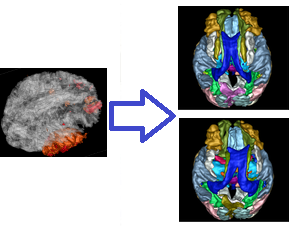
\includegraphics[scale=0.22]{./images/item0.png}} & It solves both segmentation and registration in a unified 4D framework.\\
 & \\
 \raisebox{-.5\height}{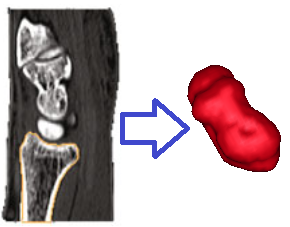
\includegraphics[scale=0.22]{./images/item1.png}} & Instead of learning 2D slices, it learns new 3D objects. \\ %\hline
 & \\
 \raisebox{-.5\height}{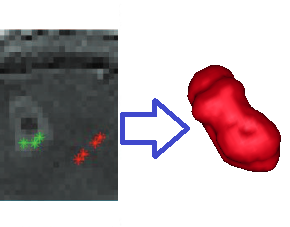
\includegraphics[scale=0.22]{./images/item2.png}} & Instead of or individual voxels, the 3D objects are better fit human visual perception due to their spatial coherence. \\
\end{tabular}
\end{center}
%\item We use one framework for segmentation and uncertainty estimation instead of using different classifiers for both tasks.
}

\section[Method]{4D Active Cut}
\frame{\frametitle{Overview of the proposed algorithm}
%% \begin{figure}
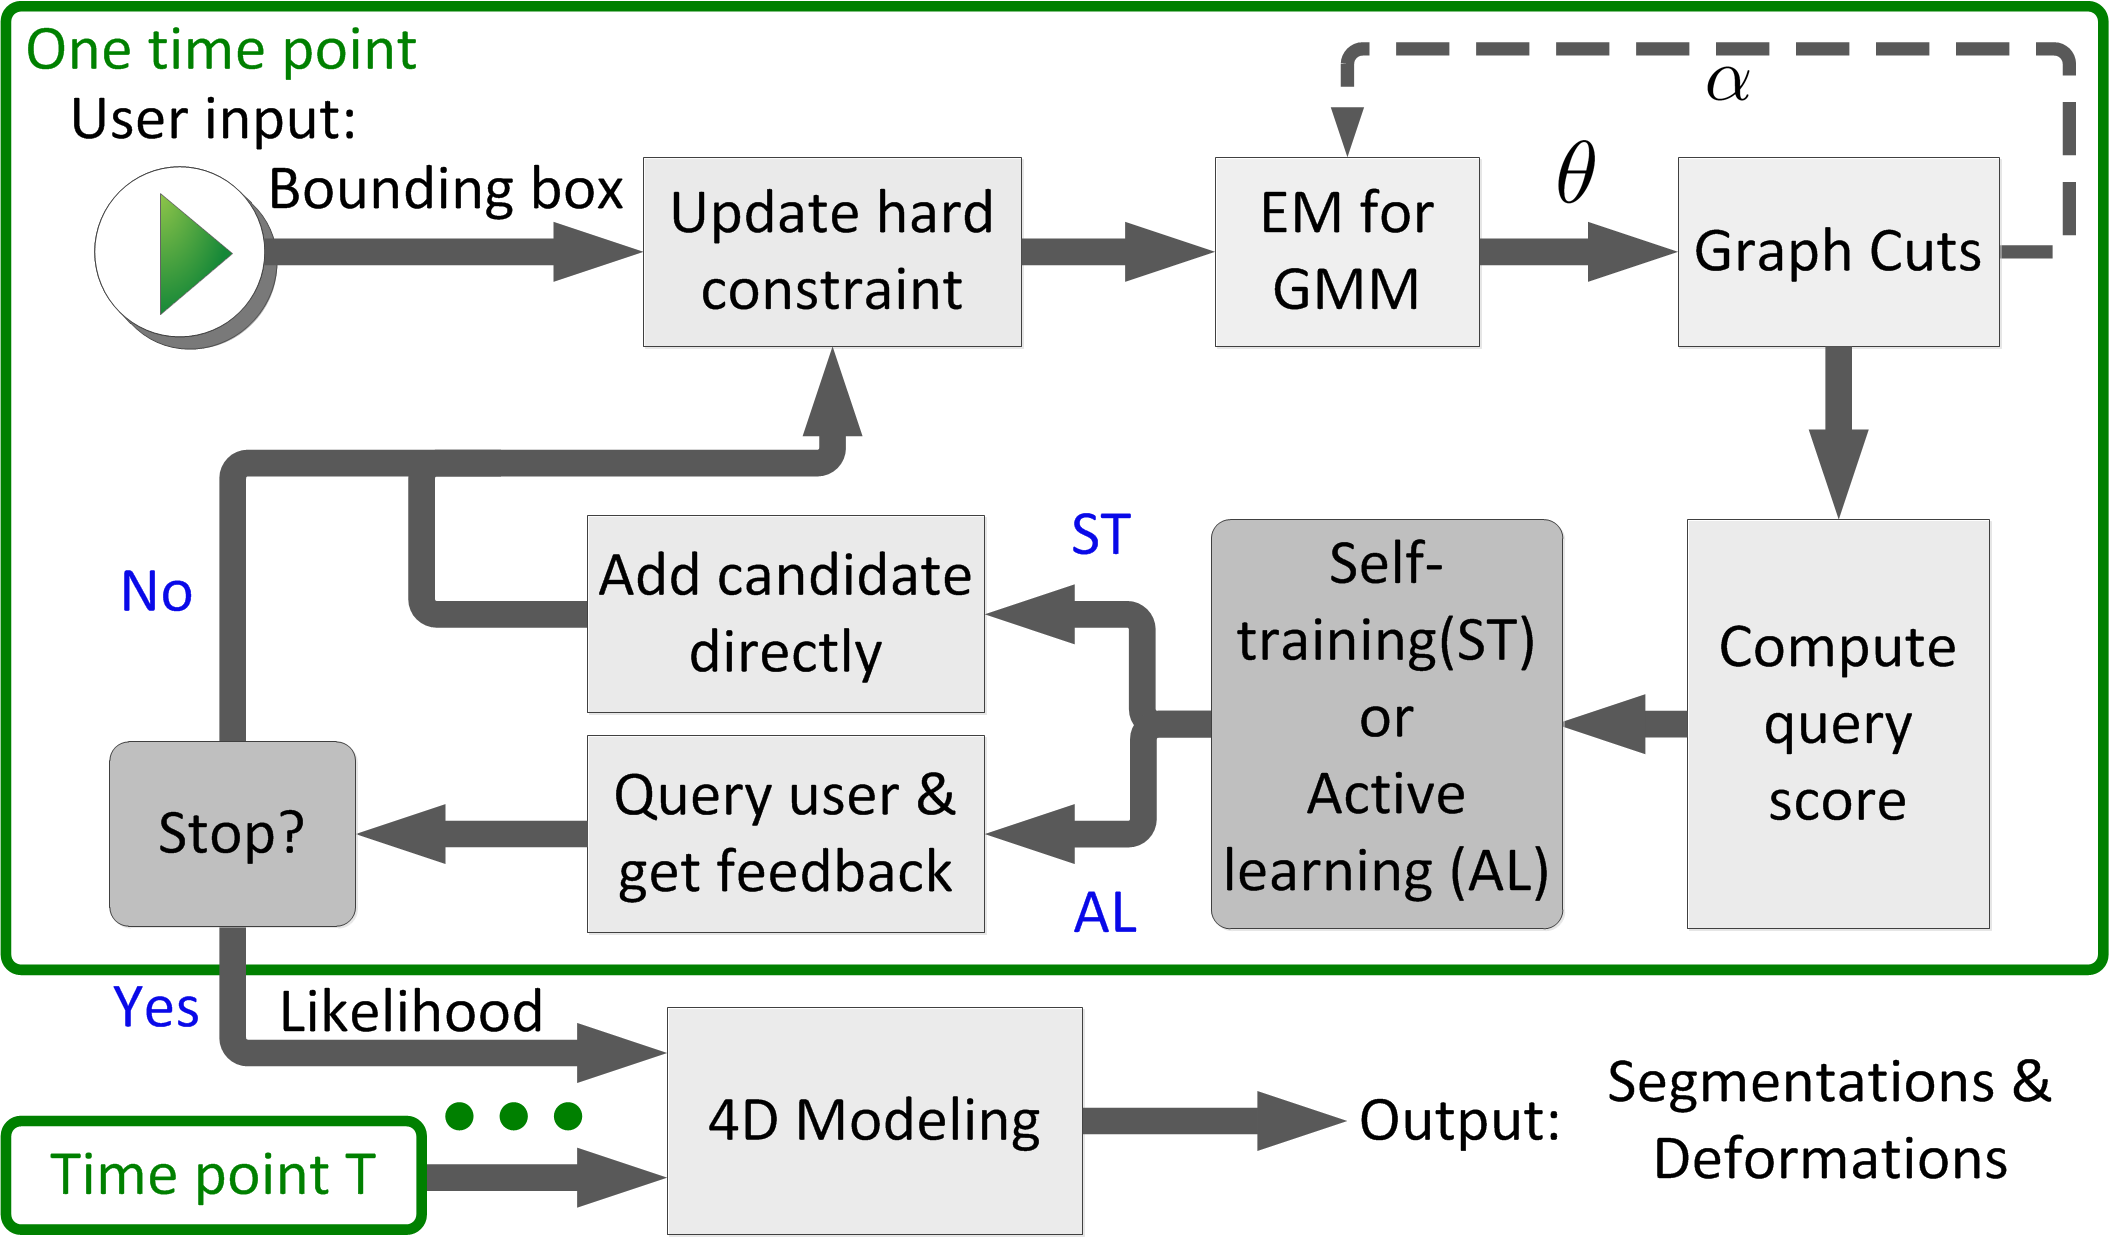
\includegraphics[width=1.0\textwidth]{./images/acLearn_flowchart.png}
%% \caption{Flowchart of the proposed algorithm.}
%% \end{figure}
}

\subsection[Guided Interaction using Active Learning]{Guided Interaction using Active Learning}

\frame{\frametitle{Within-class model}
  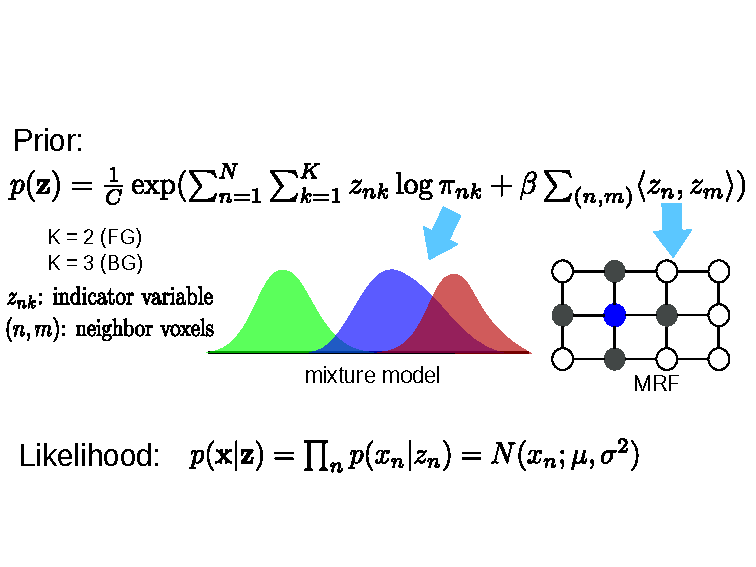
\includegraphics[width=1\textwidth]{images/prior.pdf}
}

\frame{\frametitle{Prediction Score}
Consider the case of two classes, the posterior probability for class
$C_1$ can be written as,
\begin{align*}
p(C_1 | x) = \frac{p(x | C_1) p(C_1)}{p(x | C_1) p(C_1) + p(x | C_2) p(C_2)}
 = \frac{1}{1 + \exp(-a) } = \sigma(a)
\end{align*}
where $\sigma(a)$ is the \emph{logistic sigmoid} function,
\begin{align*}
\sigma(a) = \frac{1}{1 + \exp(-a)}
\end{align*}
and
\begin{align*}
a = \ln \frac{p(x | C_1) p(C_1)}{p(x | C_2) p(C_2)}
\end{align*}
It represents the log of the ratio of probabilities $\ln [p(C_1|x)/p(C_2|x)]$
for the two classes, also known as the \emph{log odds}. \hfill \textcolor{ForestGreen}{Christopher M. Bishop, PRML}
}

\frame{\frametitle{Prediction Score}
 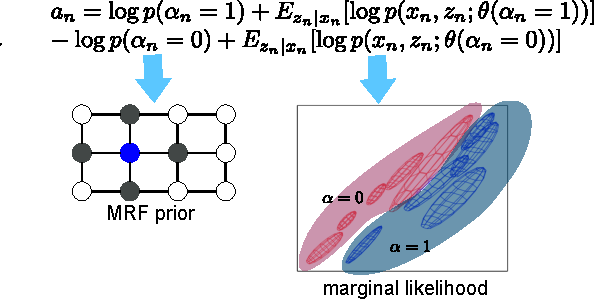
\includegraphics[width=1\textwidth]{images/logistic.pdf}
}

\frame{\frametitle{Query Score}
We obtain a binary map $\vec w$ by thresholding the predictive map at 0.5, and
identify a series of objects $R_i$ by running a connected component detection on
$\vec w$.
\begin{figure}
 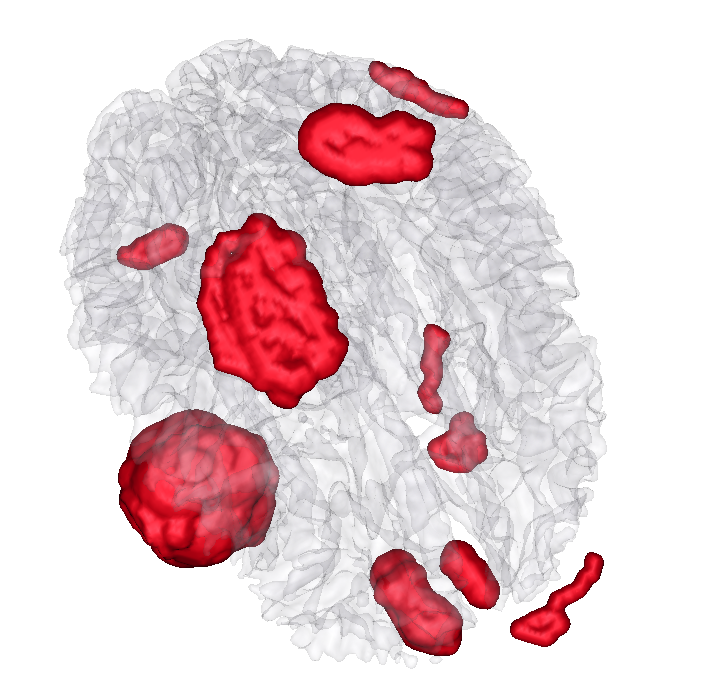
\includegraphics[width=0.5\textwidth]{images/All_candidate_patches.png}
\end{figure}
}

\frame{\frametitle{Query Score}
\begin{figure}
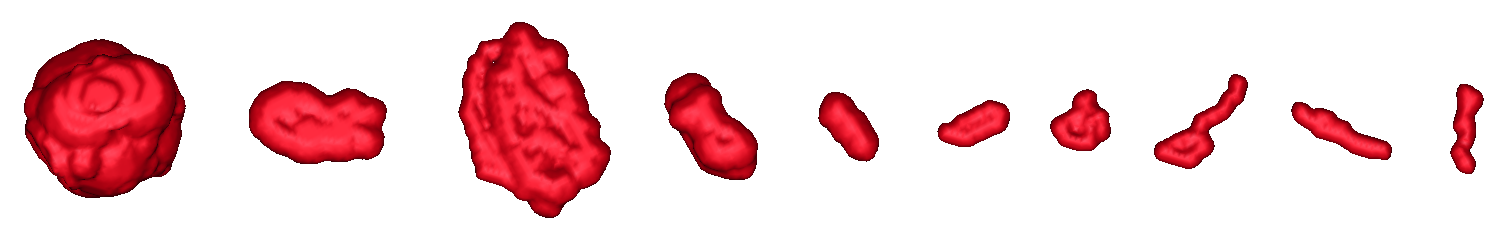
\includegraphics[width=1\textwidth]{images/All_candidate_patches_sorted.png}
\end{figure}
To select the most salient objects, we sort the objects in
decending order of the following score:
\begin{align*}
q(R_i) = \left (\sum_{n\in R_i} p(\alpha = 1| \vec x_n)  \right ) \Big /  \vert\{n: n\in \mathcal{B}(R_i) \}\vert.
\label{eq:score}
\end{align*}
$q(R_i)$ is the ratio of volume to boundary voxels. \\
 \begin{itemize}
  \item The above query score prefers objects with larger volumes of posterior probability.
  \item The score also prefers blob-like objects since such an object has large volume-surface ratio.
  \item Such criteria reflects our prior knowledge on the lesion object's shape.
\end{itemize}
}

\subsection[4D Pathological Anatomy Modeling]{4D Pathological Anatomy Modeling}
\frame{\frametitle{}
We follow the 4D pathological anatomy modeling framework of our previous work, and define $\pi_{k,t} = A_k \circ \phi_t + Q_{k,t}$,
\begin{center}
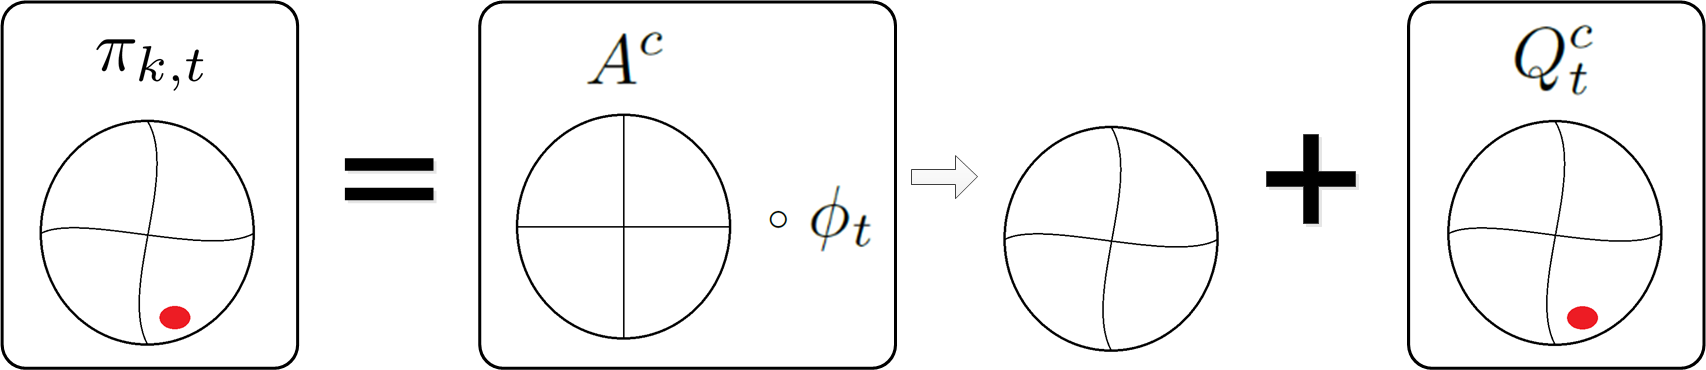
\includegraphics[width=0.8\textwidth]{./images/spatial_prior_concept_new.png}
\end{center}
where $A$ is the tissue class probability that is initially associated with the
healthy template, $\phi_t$ is the diffeomorphic deformation from time $t$ to the
atlas, and $Q_t$ is the non-diffeomorphic probabilistic change. We use alternating
gradient descent to estimate $A$, $\phi_t$ and $Q_t$ by optimizing,
\begin{align*}
\mathcal{F}(A, \phi_t, Q_t) = - \sum_{t=1}^T \mathbb{E}_{p(\mat z| \mat
  x)}[\log p (\mat z, \mat x| \theta, \pi_t)] \\
  = - \sum_{t=1}^T \sum_{i=1}^N \, \log \, \left( \, \sum_{k=1}^K \pi_{i,k,t} \, p( \mat x_{i,t} | \theta_t^c ) \, \right)
\end{align*}
}


\section{Results}
\subsection{Illustration of the iterative process}
\frame{\frametitle{1st iteration - user initialization}
\begin{figure}
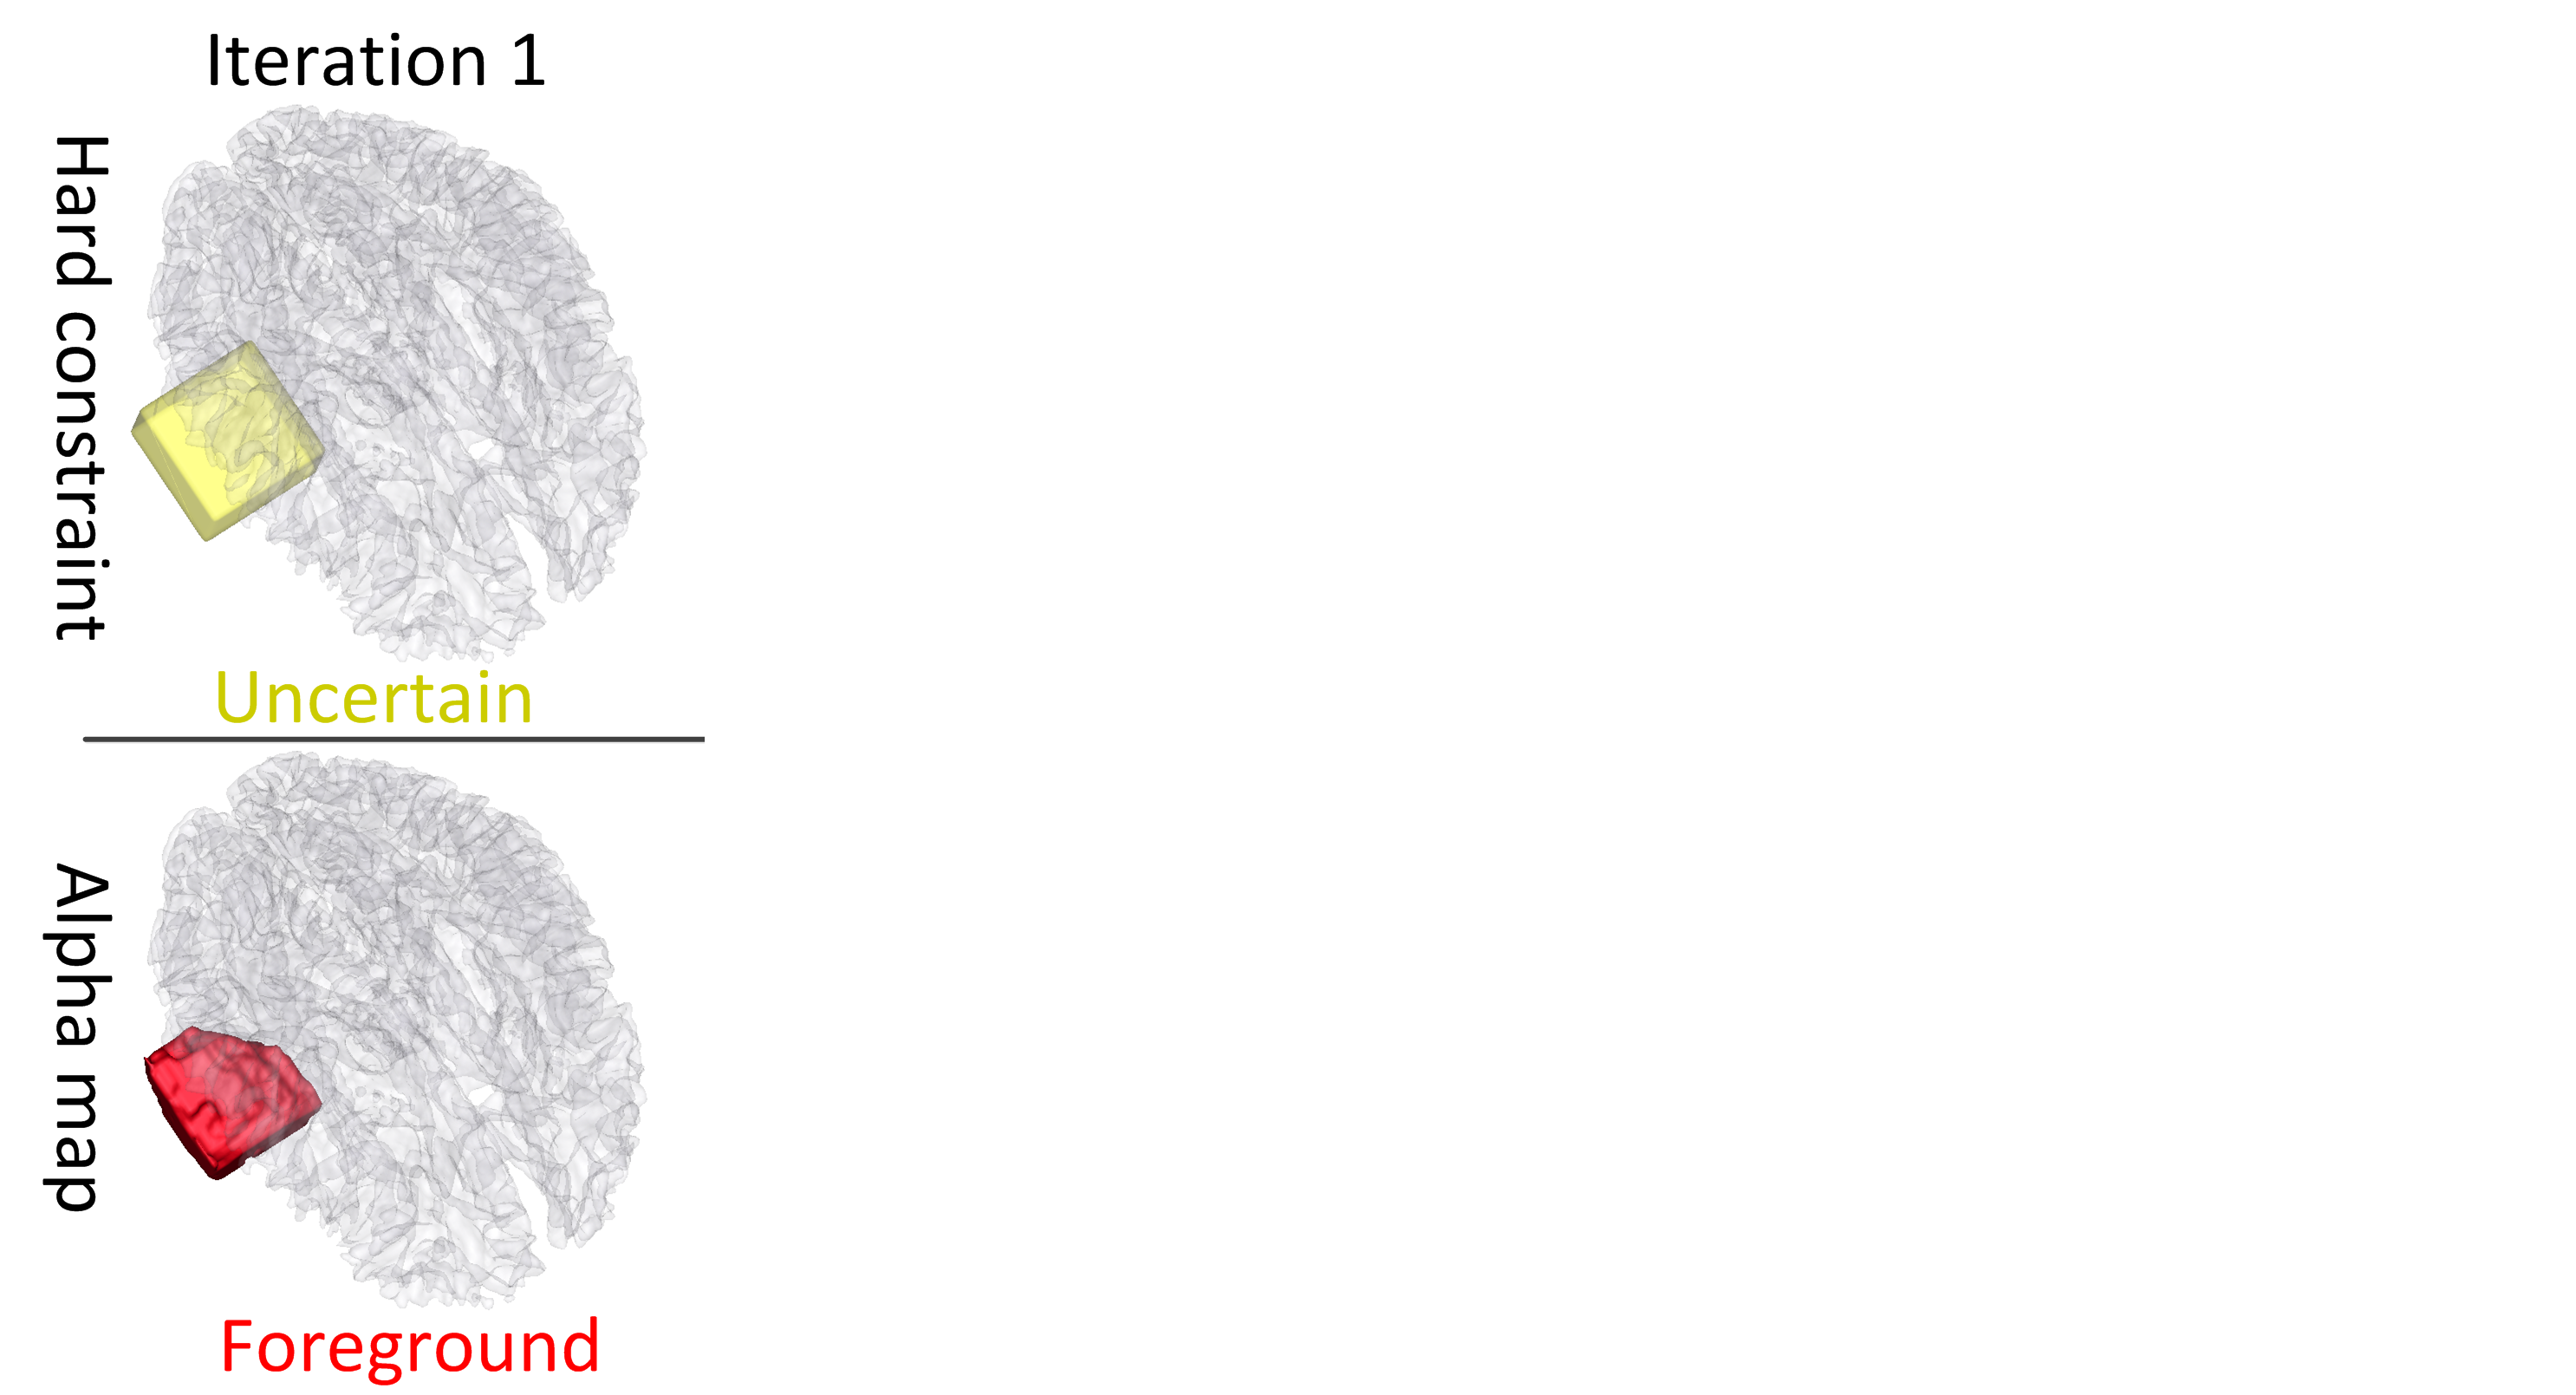
\includegraphics[width=1\textwidth]{./images/iterative_process_new_iter_1.png}
\end{figure}
}

\frame{\frametitle{2nd iteration - self training}
\begin{figure}
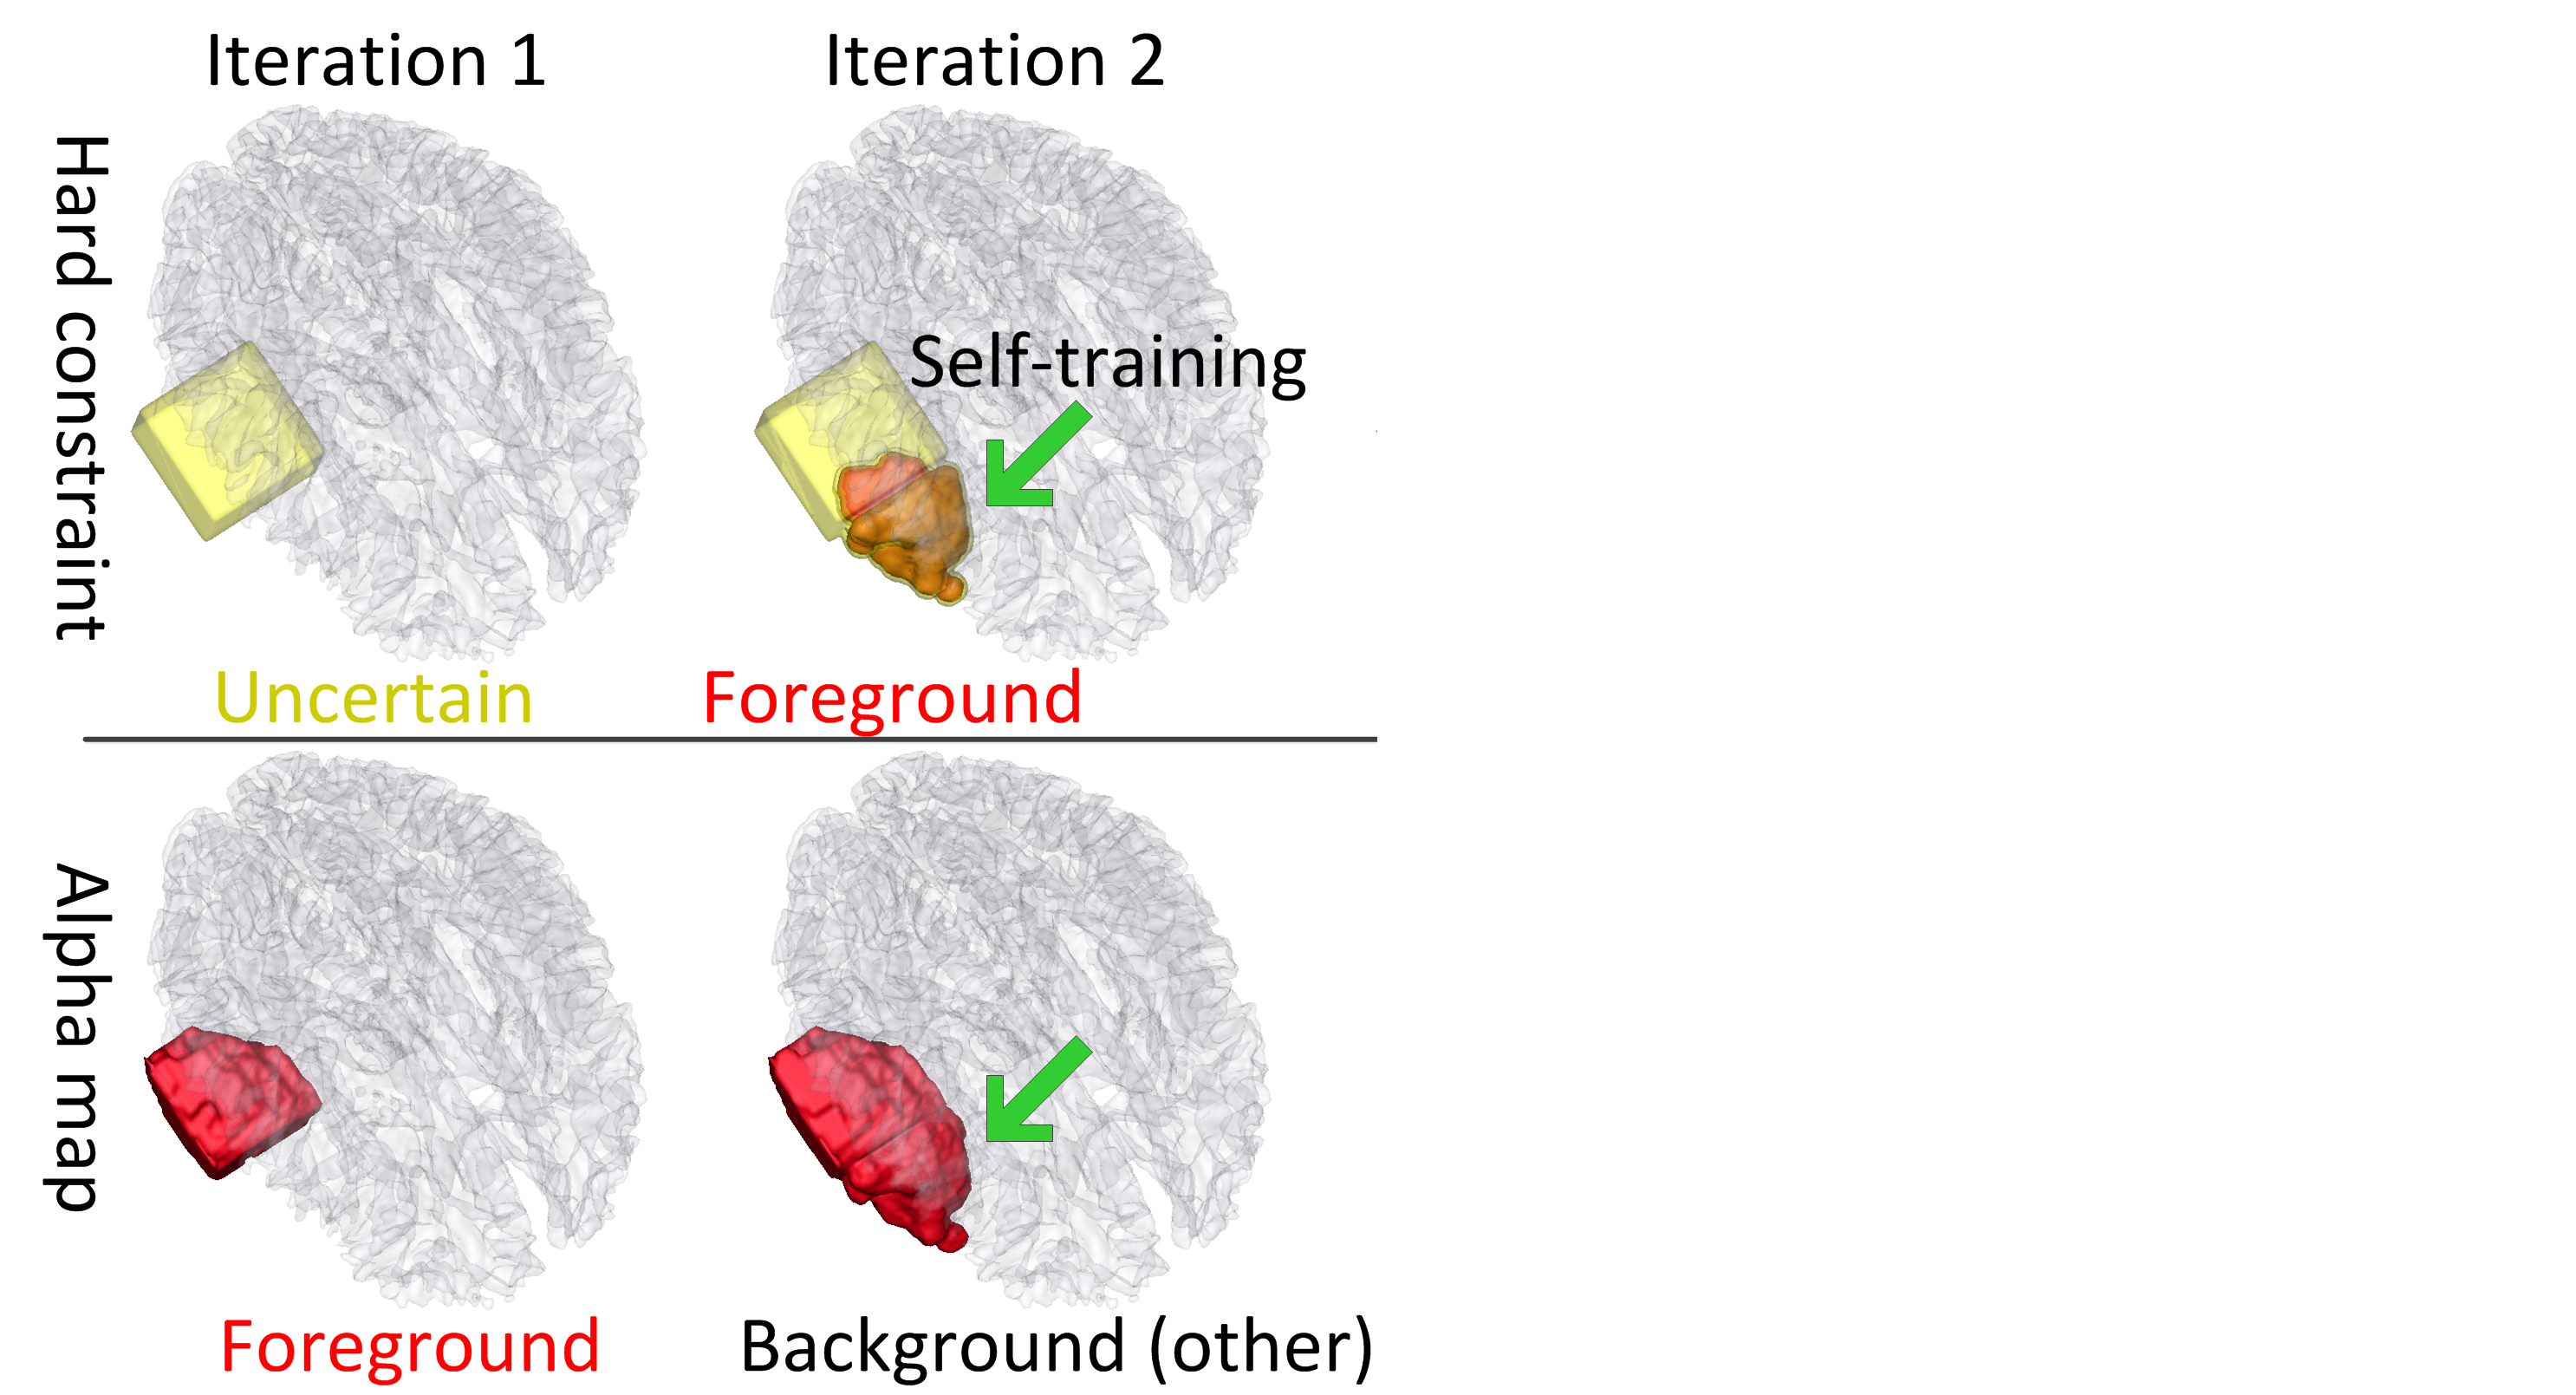
\includegraphics[width=1\textwidth]{./images/iterative_process_new_iter_2.png}
\end{figure}
}

\frame{\frametitle{3rd iteration - active learning}
\begin{figure}
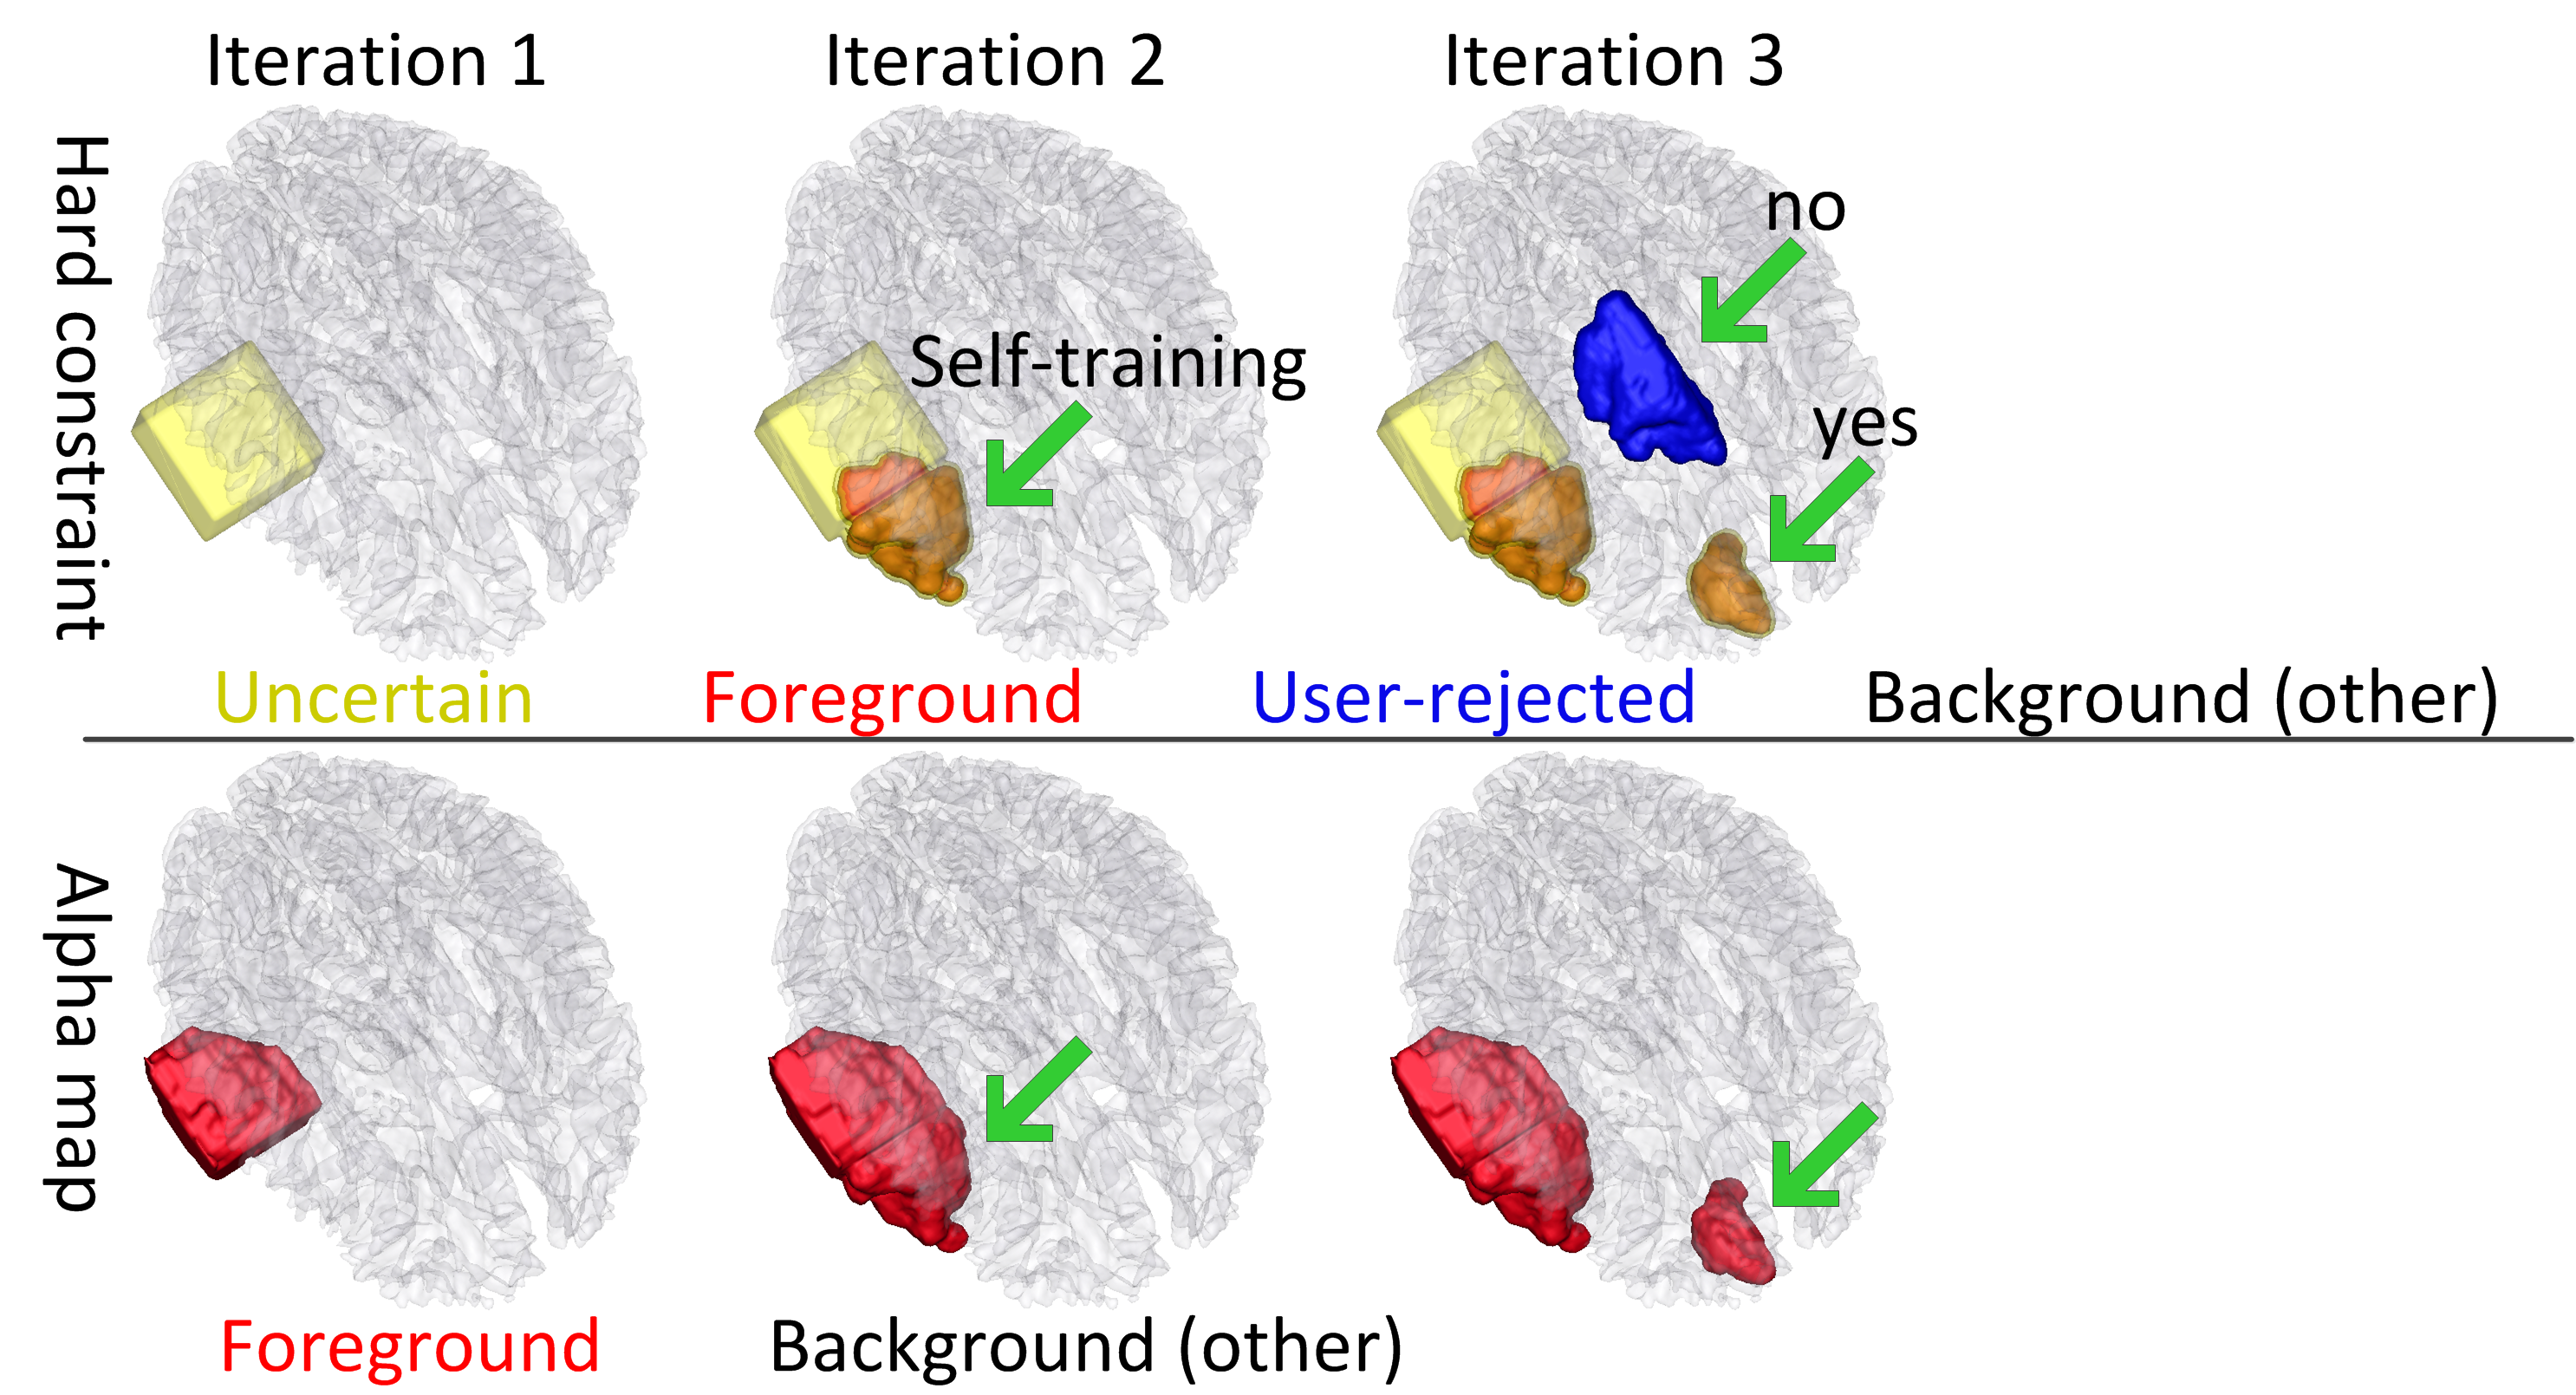
\includegraphics[width=1\textwidth]{./images/iterative_process_new_iter_3.png}
\end{figure}
}

\frame{\frametitle{4th iteration - active learning}
\begin{figure}
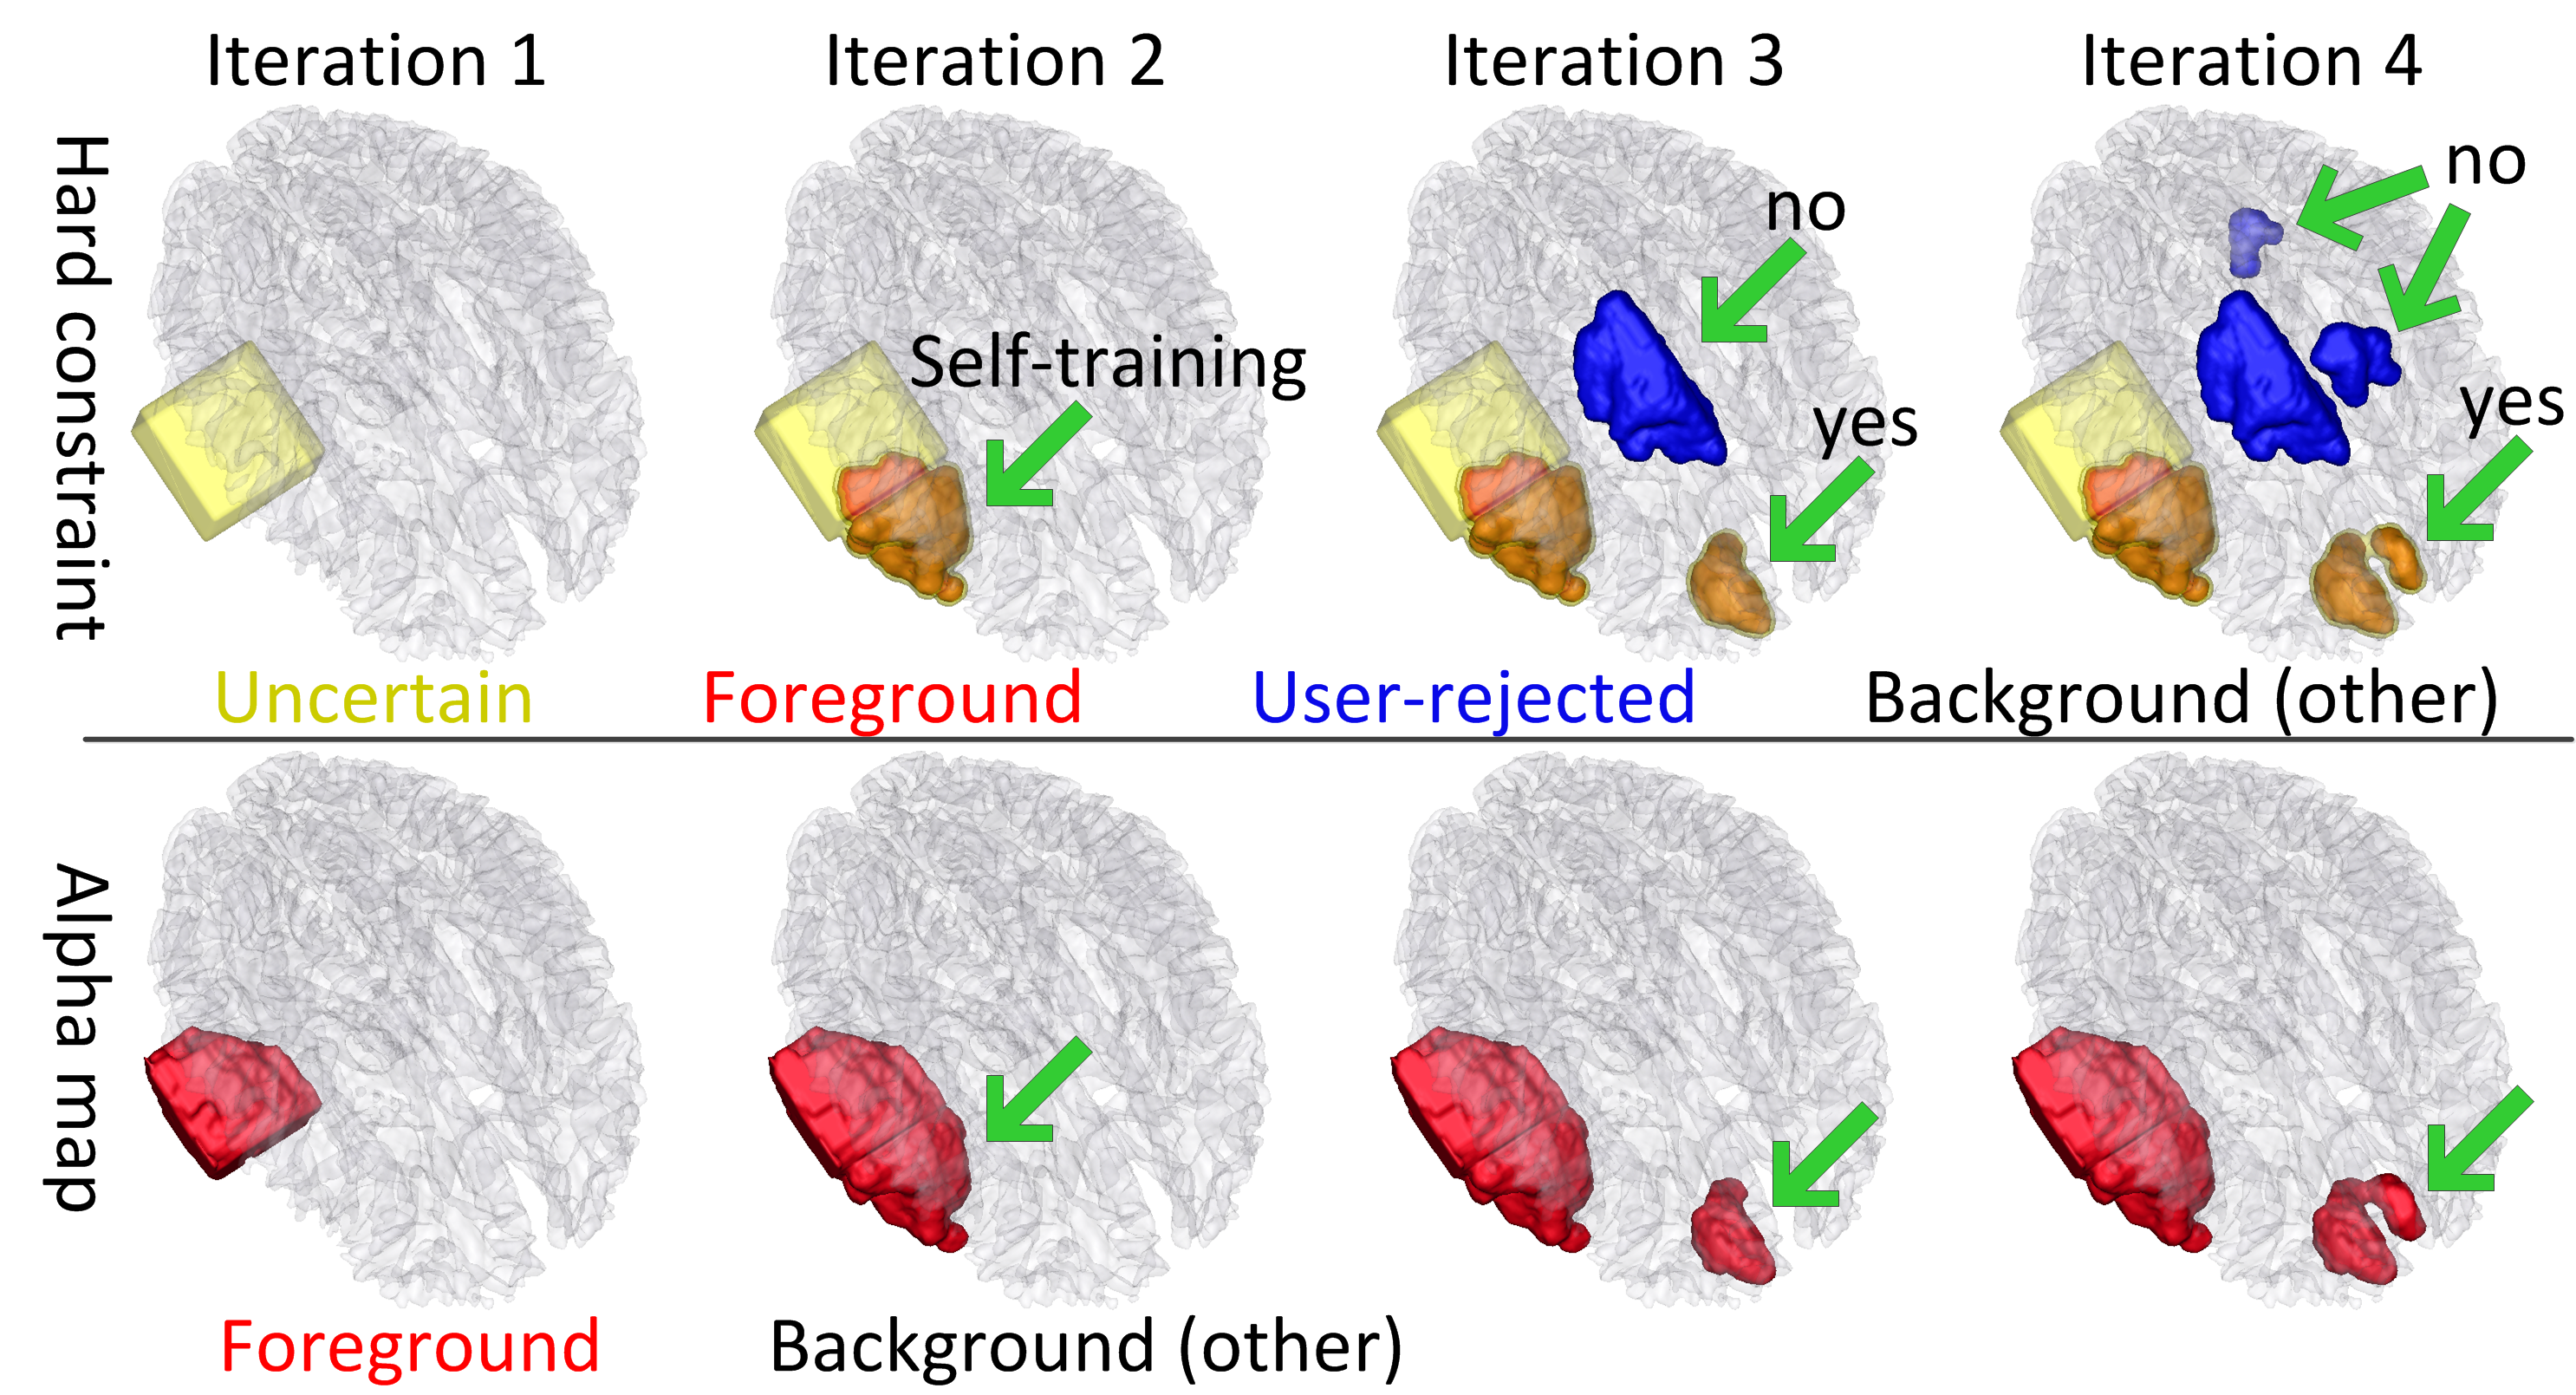
\includegraphics[width=1\textwidth]{./images/iterative_process_new.png}
\end{figure}
}

\subsection{Qualitative and quantitative comparison}
\frame{\frametitle{Qualitative comparison}
\begin{figure}
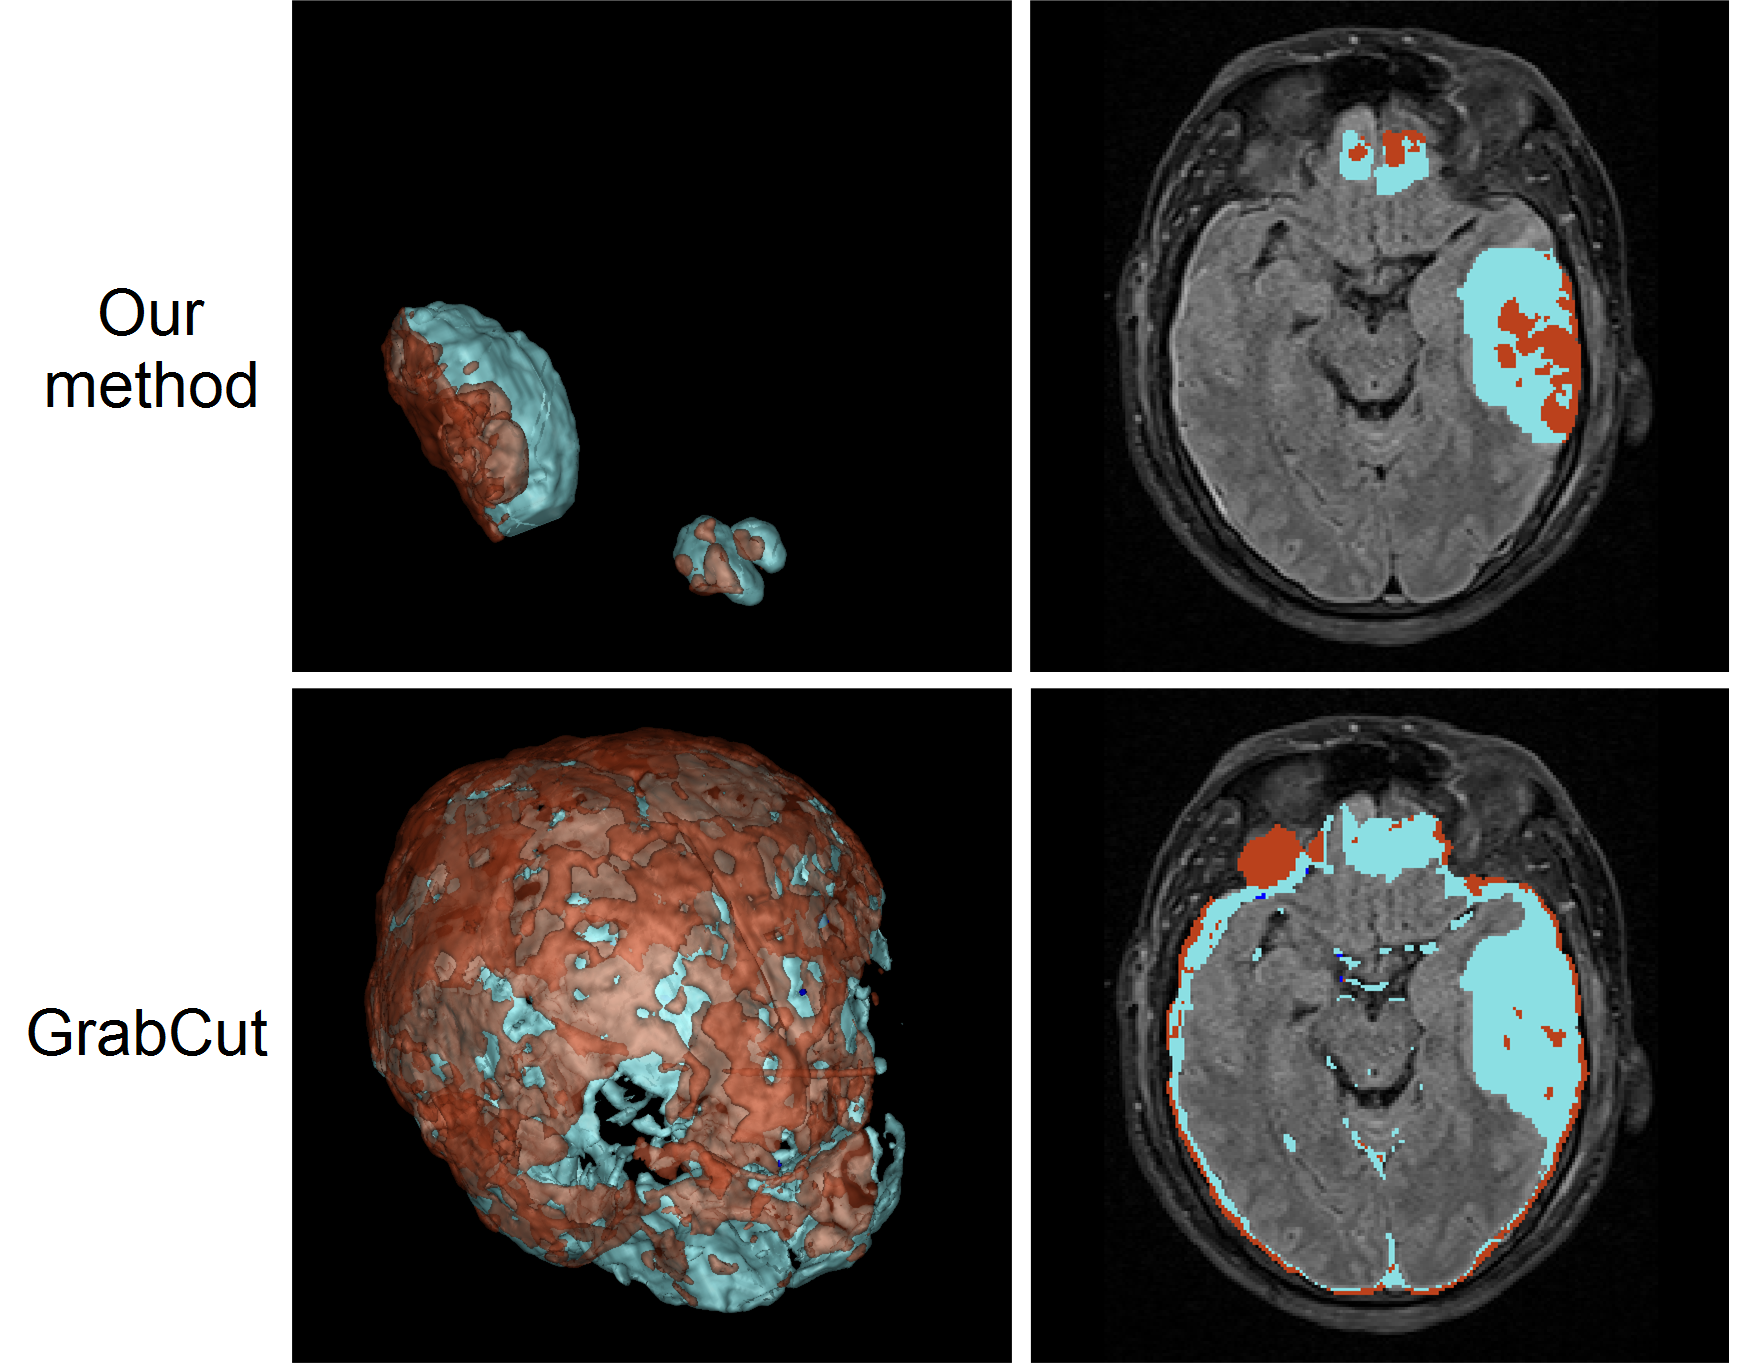
\includegraphics[width=0.99\textwidth]{./images/qualitative_comp.png}
\end{figure}
}

\frame{\frametitle{Quantitative comparison}
\begin{table} [ht]
%\begin{center}
\centering
\begin{tabular}{c|cc|cc|c}
\hline
 &  \multicolumn{2}{c}{Baseline} &  \multicolumn{3}{|c}{4D active cut}\\
\cline{2-6}
\multirow{1}{*}{Subject}  & NHL & HL & NHL & HL & UI\\

I  & 0.2503 & 0.0613  & 0.6349 & 0.5698 & 5\\ %\hline
II & 0.3269 & -  & 0.6910 & -   & 4 \\ %\hline
III  & 0.1311 & 0.2288   & 0.4512 & 0.4840 & 6 \\ %\hline
IV   & 0.0918 & 0.0998   & 0.3503 & 0.1153 & 5 \\ \hline
\end{tabular}
\caption{ Dice values comparing \emph{4D active cut} and GrabCut to ground
  truth. HL and NHL are acute hemorrhagic and non-hemorrhagic lesions. UI
  denotes the number of interactions a user performed using \emph{4D active cut}.
  Subject II has no ground truth for HL due to the lack of GRE modality.}
\label{tab:DiceResult}
\end{table}
}

\frame{\frametitle{Result of 4D modeling}
\begin{figure}
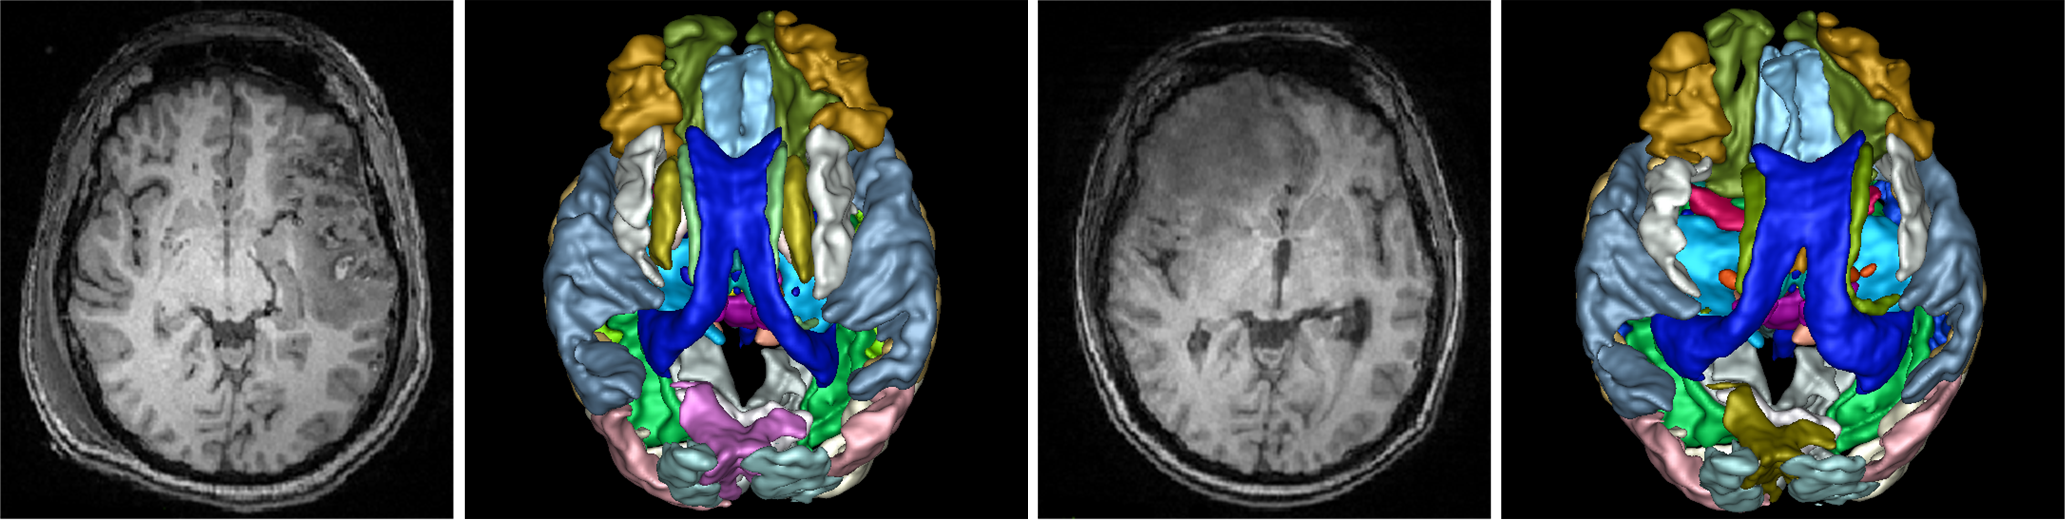
\includegraphics[width=0.9\textwidth]{./images/parcellation.png}
\caption{Result of mapping parcellation labels associated with the healthy
  template to each time point. The left two images are the T1 reference TBI image at acute stage and mapped parcellations, and the right two images are the same at chronic stage.}
\end{figure}
}

\section{Conclusions}

\frame{\frametitle{Conclusions}
Advantages of the proposed framework
\begin{itemize}
\item It actively query users candidate patches instead of passively wait for user correction.
\item It can detect multiple lesion objects with minimal user input.
\item It is robust given inaccurate user initialization.
\item It does 4D modeling instead of only 3D segmentation.
\end{itemize}
}

\frame{\frametitle{Future work}
\begin{itemize}
\item Explore integration of active learning and 4D modeling.
\item Validation and verification on other image data presenting pathologies.
\end{itemize}
}

\frame{\frametitle{Thanks!}
\begin{center}
{\LARGE Thank you for your attention!}
\end{center}
\begin{center}
{\LARGE Questions?}
\end{center}
}

\frame{\frametitle{Variational Inference}
  \begin{columns}[c]
    \begin{column}{0.6\textwidth}

      \begin{itemize}
        \item Search $p(z | x)$ in subspace: $Q(z) = \prod_n q_n(z_n)$.
        \item   $\log p(z_{nk}) = z_{nk} \pi_{nk} + \sum_{m\in \mathcal{N}(n)}\langle \mathbb{E}(\vec z_m), \vec z_n \rangle + \log \mathcal{N} (\vec x_n; \theta(\vec z_n))$
        \item $\mathbb{E}(z_{nk}) = p(z_{nk} = 1)$ for binary variable
          $z_{nk}$. Save $\mathbb{E}(z_{nk})$ for updateing other nodes.
        \end{itemize}
      \end{column}

    \begin{column}{0.4\textwidth}
      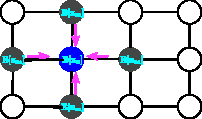
\includegraphics[width=1\textwidth]{images/variational}
    \end{column}

  \end{columns}

}
\end{document}
